% begin module cardioid-ex7
\begin{frame}
\begin{example}[Example 7, p. 679]
Sketch the curve $r = 1 + \sin \theta$.
\begin{columns}[c]
\column{.3\textwidth}
\ \only<handout:0| 1>{%
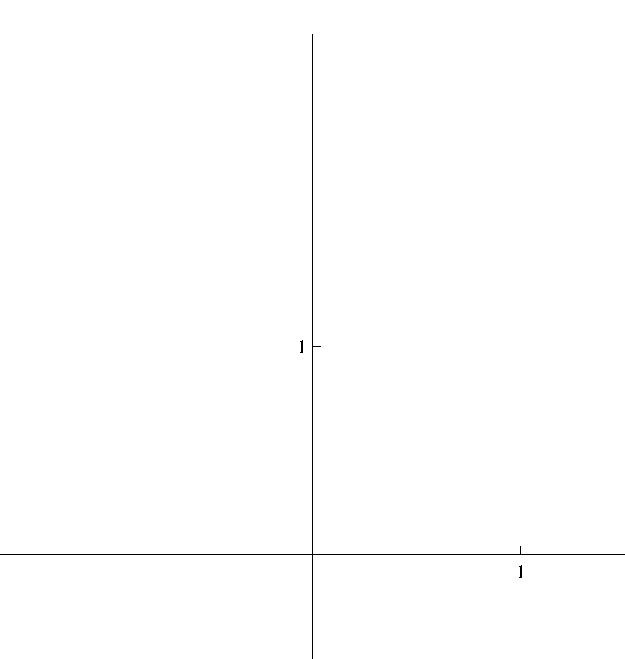
\includegraphics[height=3.6cm]{polar-curves/pictures/11-03-ex7a.pdf}%
}%
\only<handout:0| 2>{%
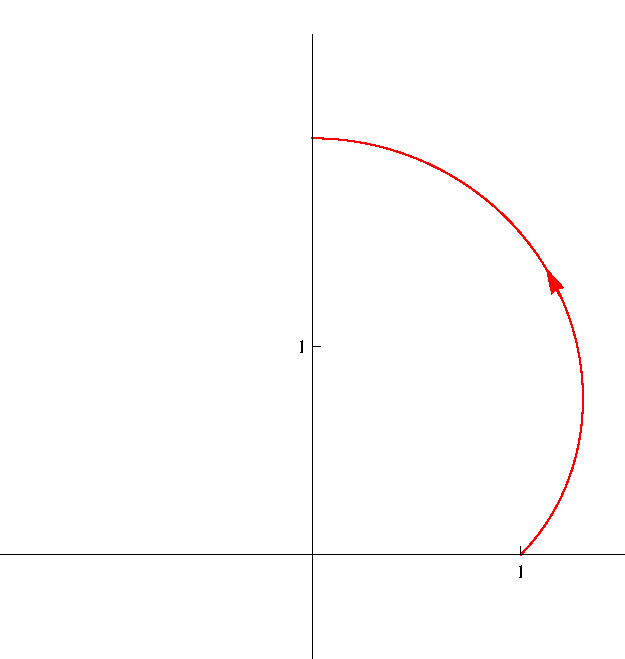
\includegraphics[height=3.6cm]{polar-curves/pictures/11-03-ex7b.pdf}%
}%
\only<handout:0| 3>{%
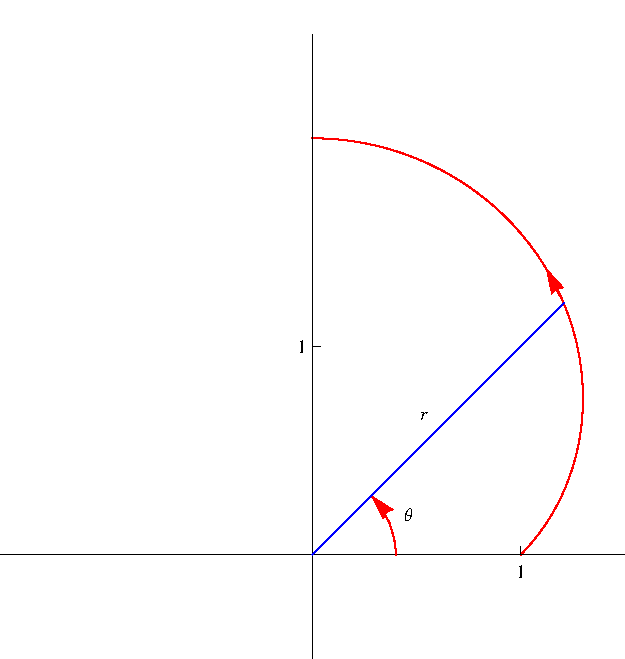
\includegraphics[height=3.6cm]{polar-curves/pictures/11-03-ex7ba.pdf}%
}%
\only<handout:0| 4>{%
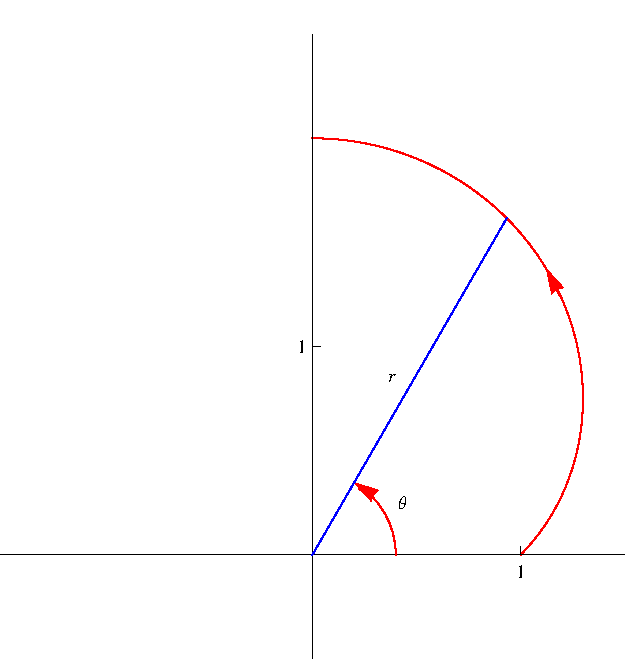
\includegraphics[height=3.6cm]{polar-curves/pictures/11-03-ex7bb.pdf}%
}%
\only<handout:0| 5>{%
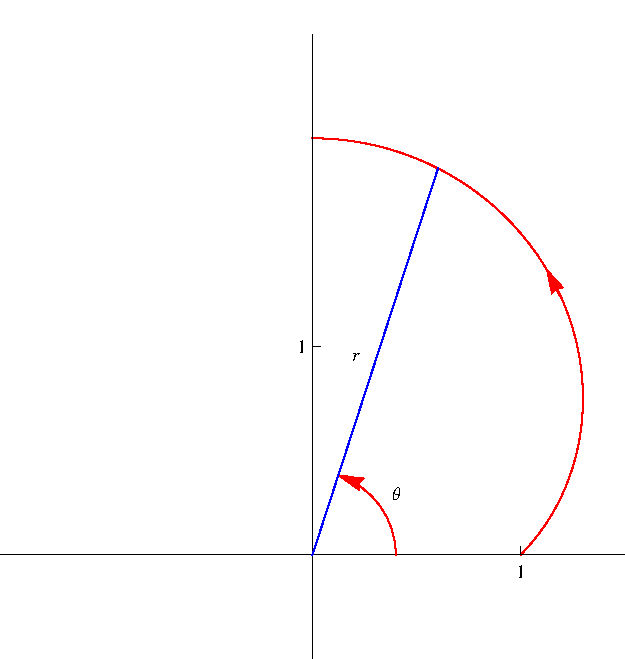
\includegraphics[height=3.6cm]{polar-curves/pictures/11-03-ex7bc.pdf}%
}%
\only<handout:0| 6>{%
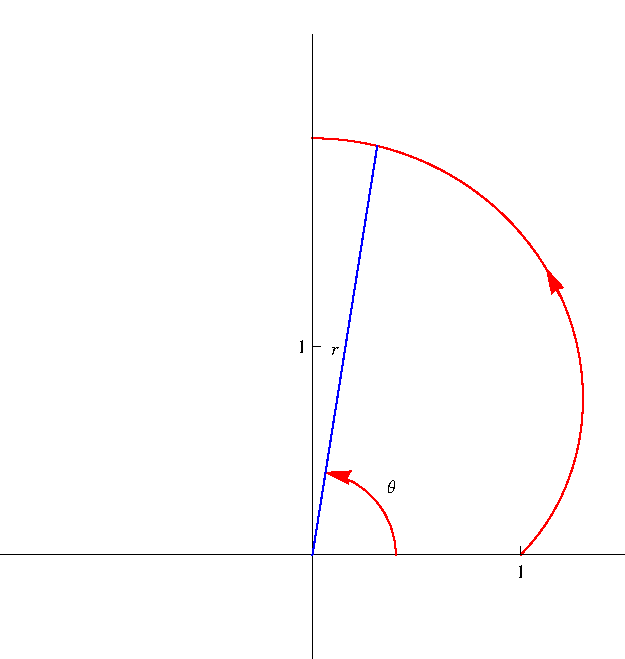
\includegraphics[height=3.6cm]{polar-curves/pictures/11-03-ex7bd.pdf}%
}%
\only<handout:0| 7>{%
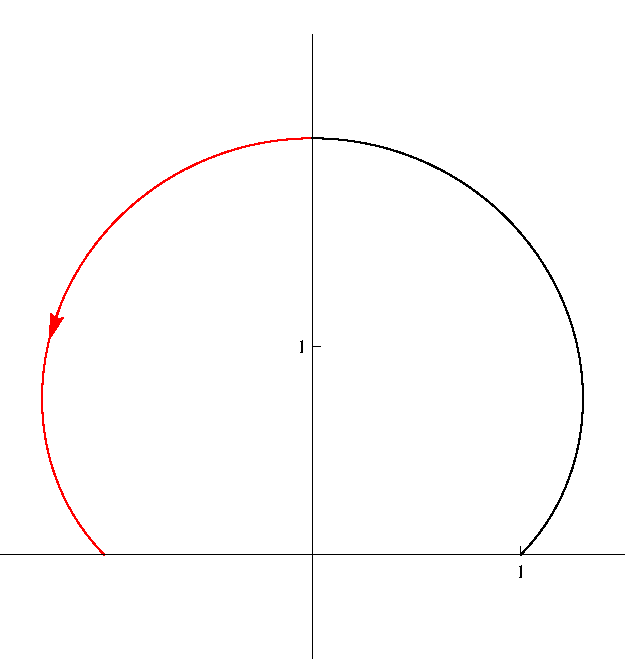
\includegraphics[height=3.6cm]{polar-curves/pictures/11-03-ex7c.pdf}%
}%
\only<handout:0| 8>{%
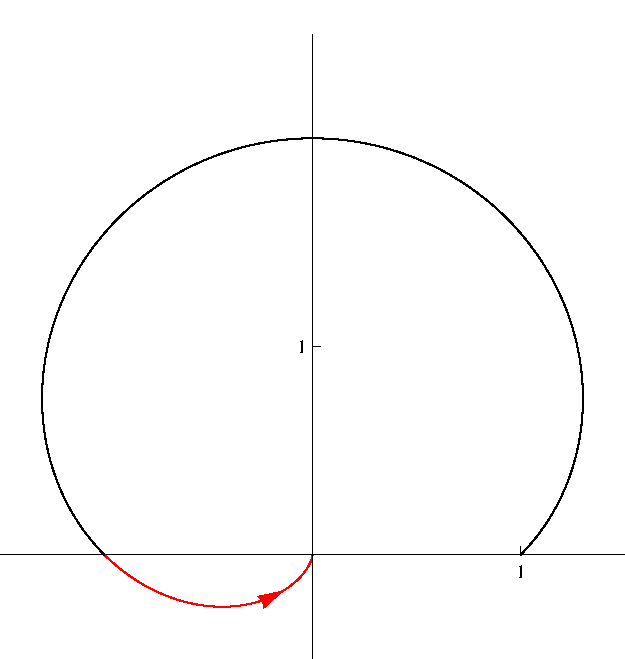
\includegraphics[height=3.6cm]{polar-curves/pictures/11-03-ex7d.pdf}%
}%
\only<9->{%
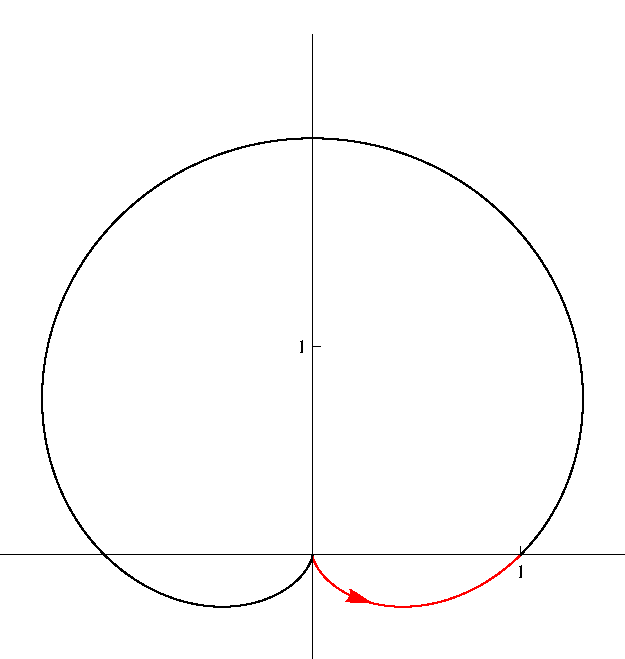
\includegraphics[height=3.6cm]{polar-curves/pictures/11-03-ex7e.pdf}%
}%
\column{.7\textwidth}
\ \only<handout:0| 1>{%
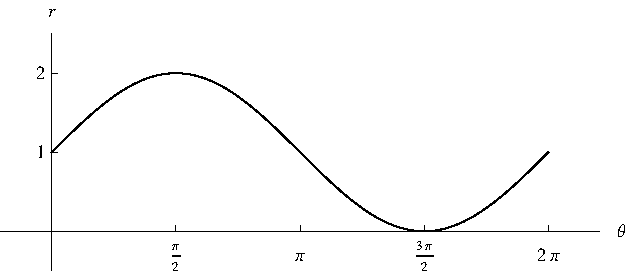
\includegraphics[height=3.6cm]{polar-curves/pictures/11-03-ex7helpera.pdf}%
}%
\only<handout:0| 2>{%
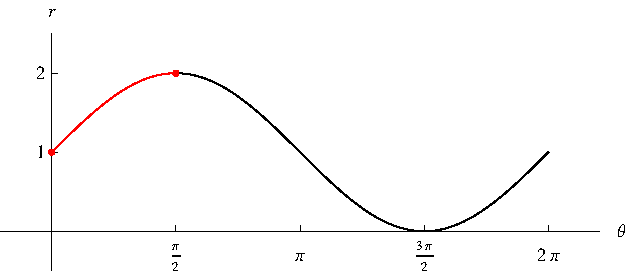
\includegraphics[height=3.6cm]{polar-curves/pictures/11-03-ex7helperb.pdf}%
}%
\only<handout:0| 3>{%
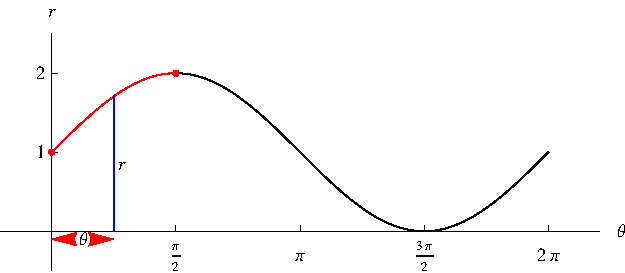
\includegraphics[height=3.6cm]{polar-curves/pictures/11-03-ex7helperba.pdf}%
}%
\only<handout:0| 4>{%
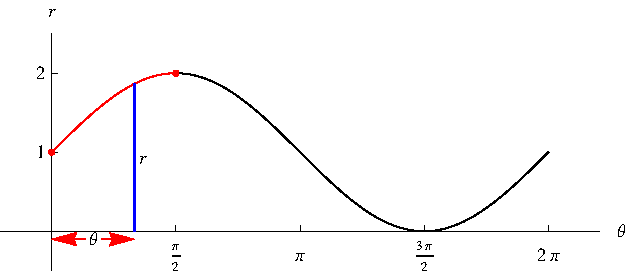
\includegraphics[height=3.6cm]{polar-curves/pictures/11-03-ex7helperbb.pdf}%
}%
\only<handout:0| 5>{%
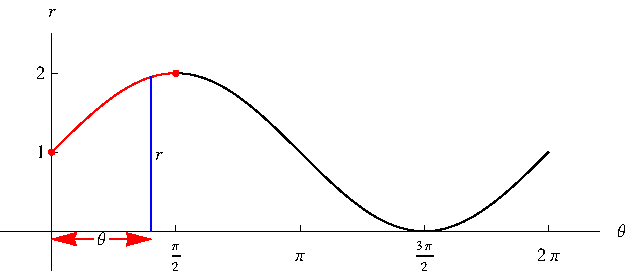
\includegraphics[height=3.6cm]{polar-curves/pictures/11-03-ex7helperbc.pdf}%
}%
\only<handout:0| 6>{%
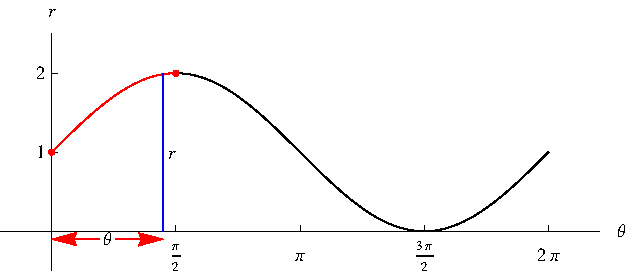
\includegraphics[height=3.6cm]{polar-curves/pictures/11-03-ex7helperbd.pdf}%
}%
\only<handout:0| 7>{%
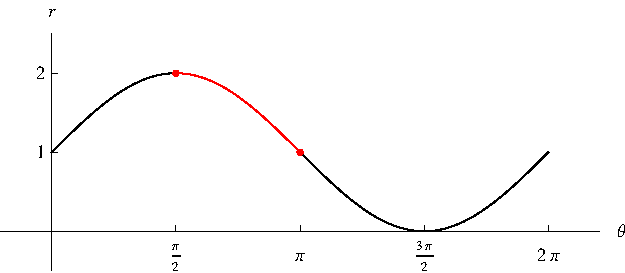
\includegraphics[height=3.6cm]{polar-curves/pictures/11-03-ex7helperc.pdf}%
}%
\only<handout:0| 8>{%
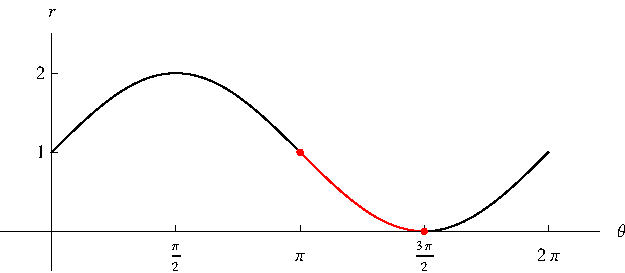
\includegraphics[height=3.6cm]{polar-curves/pictures/11-03-ex7helperd.pdf}%
}%
\only<9->{%
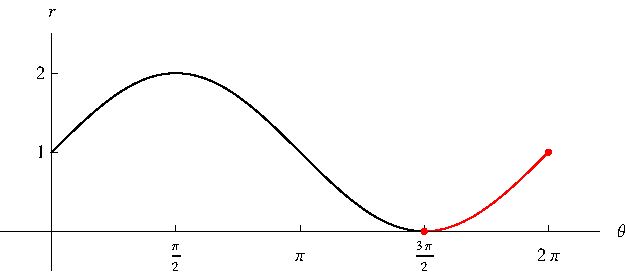
\includegraphics[height=3.6cm]{polar-curves/pictures/11-03-ex7helpere.pdf}%
}%
\end{columns}
\end{example}
\end{frame}
% end module cardioid-ex7
